\documentclass[handout,nooutcomes,noauthor]{ximera}

\graphicspath{  
{./}
{./whoAreYou/}
{./drawingWithTheTurtle/}
{./bisectionMethod/}
{./circles/}
{./anglesAndRightTriangles/}
{./lawOfSines/}
{./lawOfCosines/}
{./plotter/}
{./staircases/}
{./pitch/}
{./qualityControl/}
{./symmetry/}
{./nGonBlock/}
}


%% page layout
\usepackage[cm,headings]{fullpage}
\raggedright
\setlength\headheight{13.6pt}


%% fonts
\usepackage{euler}

\usepackage{FiraMono}
\renewcommand\familydefault{\ttdefault} 
\usepackage[defaultmathsizes]{mathastext}
\usepackage[htt]{hyphenat}

\usepackage[T1]{fontenc}
\usepackage[scaled=1]{FiraSans}

%\usepackage{wedn}
\usepackage{pbsi} %% Answer font


\usepackage{cancel} %% strike through in pitch/pitch.tex


%% \usepackage{ulem} %% 
%% \renewcommand{\ULthickness}{2pt}% changes underline thickness

\tikzset{>=stealth}

\usepackage{adjustbox}

\setcounter{titlenumber}{-1}

%% journal style
\makeatletter
\newcommand\journalstyle{%
  \def\activitystyle{activity-chapter}
  \def\maketitle{%
    \addtocounter{titlenumber}{1}%
                {\flushleft\small\sffamily\bfseries\@pretitle\par\vspace{-1.5em}}%
                {\flushleft\LARGE\sffamily\bfseries\thetitlenumber\hspace{1em}\@title \par }%
                {\vskip .6em\noindent\textit\theabstract\setcounter{question}{0}\setcounter{sectiontitlenumber}{0}}%
                    \par\vspace{2em}
                    \phantomsection\addcontentsline{toc}{section}{\thetitlenumber\hspace{1em}\textbf{\@title}}%
                     }}
\makeatother



%% thm like environments
\let\question\relax
\let\endquestion\relax

\newtheoremstyle{QuestionStyle}{\topsep}{\topsep}%%% space between body and thm
		{}                      %%% Thm body font
		{}                              %%% Indent amount (empty = no indent)
		{\bfseries}            %%% Thm head font
		{)}                              %%% Punctuation after thm head
		{ }                           %%% Space after thm head
		{\thmnumber{#2}\thmnote{ \bfseries(#3)}}%%% Thm head spec
\theoremstyle{QuestionStyle}
\newtheorem{question}{}



\let\freeResponse\relax
\let\endfreeResponse\relax

%% \newtheoremstyle{ResponseStyle}{\topsep}{\topsep}%%% space between body and thm
%% 		{\wedn\bfseries}                      %%% Thm body font
%% 		{}                              %%% Indent amount (empty = no indent)
%% 		{\wedn\bfseries}            %%% Thm head font
%% 		{}                              %%% Punctuation after thm head
%% 		{3ex}                           %%% Space after thm head
%% 		{\underline{\underline{\thmname{#1}}}}%%% Thm head spec
%% \theoremstyle{ResponseStyle}

\usepackage[tikz]{mdframed}
\mdfdefinestyle{ResponseStyle}{leftmargin=1cm,linecolor=black,roundcorner=5pt,
, font=\bsifamily,}%font=\wedn\bfseries\upshape,}


\ifhandout
\NewEnviron{freeResponse}{}
\else
%\newtheorem{freeResponse}{Response:}
\newenvironment{freeResponse}{\begin{mdframed}[style=ResponseStyle]}{\end{mdframed}}
\fi



%% attempting to automate outcomes.

%% \newwrite\outcomefile
%%   \immediate\openout\outcomefile=\jobname.oc
%% \renewcommand{\outcome}[1]{\edef\theoutcomes{\theoutcomes #1~}%
%% \immediate\write\outcomefile{\unexpanded{\outcome}{#1}}}

%% \newcommand{\outcomelist}{\begin{itemize}\theoutcomes\end{itemize}}

%% \NewEnviron{listOutcomes}{\small\sffamily
%% After answering the following questions, students should be able to:
%% \begin{itemize}
%% \BODY
%% \end{itemize}
%% }
\usepackage[tikz]{mdframed}
\mdfdefinestyle{OutcomeStyle}{leftmargin=2cm,rightmargin=2cm,linecolor=black,roundcorner=5pt,
, font=\small\sffamily,}%font=\wedn\bfseries\upshape,}
\newenvironment{listOutcomes}{\begin{mdframed}[style=OutcomeStyle]After answering the following questions, students should be able to:\begin{itemize}}{\end{itemize}\end{mdframed}}



%% my commands

\newcommand{\snap}{{\bfseries\itshape\textsf{Snap!}}}
\newcommand{\flavor}{\link[\snap]{https://snap.berkeley.edu/}}
\newcommand{\mooculus}{\textsf{\textbf{MOOC}\textnormal{\textsf{ULUS}}}}


\usepackage{tkz-euclide}
\tikzstyle geometryDiagrams=[rounded corners=.5pt,ultra thick,color=black]
\colorlet{penColor}{black} % Color of a curve in a plot



\ifhandout\newcommand{\mynewpage}{\newpage}\else\newcommand{\mynewpage}{}\fi

\title{Life on a cone}

\author{Jenny Sheldon \and Bart Snapp}

\begin{document}
\begin{abstract}
  Geometry changes when we work on different surfaces.
\end{abstract}
\maketitle


\begin{listOutcomes}
\item 
\end{listOutcomes}


\mynewpage



\begin{question}
  
\end{question}

\mynewpage


\begin{question}
\end{question}

\mynewpage


\begin{question}
 \end{question}


%% \begin{prob}
%% Put a dot at the center of a blank sheet of paper and call it $\vec{o}$.
%% Use a protractor to draw an angle of $50^\circ$ with vertex at the
%% point $\vec{o}$ and sides extending all the way out to the edge of the
%% paper.  Cut the paper along one side of the angle and one side only.
%% Make a cone by moving the cut edge to the other side of the angle you
%% drew.  This cone (extended infinitely) is your universe.
%% \end{prob}


%% \begin{prob}
%% Make a triangle in your universe that surrounds $\vec{o}$. To do this,
%% unfold your universe and lay it out flat on the desk and make the
%% sides with your ruler.  When a side gets to the cut side of your
%% angle, put the other side of the angle on top and keep going.
%% \end{prob}

%% \begin{prob}
%% You measure angles on your universe by laying the paper out flat and
%% measuring the angles on the paper. Measure the angles in your
%% triangle.  What do they sum to?
%% \end{prob}


%% \begin{prob}
%% Repeat the problems above, but this time cut an angle of $40^\circ$ to
%% make your cone. What do you notice?
%% \end{prob}

%% Let's see if we can explain this. Do you know who is eager to help
%% you? That's right: Louie Llama.
%% \[
%% 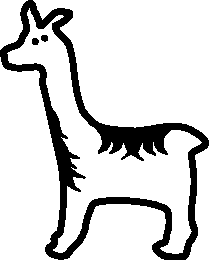
\includegraphics[height=1in]{../graphics/llama.pdf}
%% \]

%% \begin{prob}
%% Take your triangle and denote the measure of its angles as $a$, $b$,
%% and $c$. We would like to parade Louie around the triangle. There is
%% only one catch: What happens to Louie when he passes over the ``cut?''
%% Draw some pictures and see if you can figure it out.
%% \end{prob}

%% Start Louie Llama out along a side adjacent to the angle of measure
%% $a$. He should be on the outside of the triangle, his feet should be
%% pointing toward the triangle, and his face should be pointing toward
%% the angle of measure $b$. Continue this process and walk him all
%% around the triangle. When he gets to the ``cut'' put the paper
%% together, and let him continue his walk.

%% \begin{prob} 
%% Through what angle does Louie rotate when he strolls around a vertex?
%% \end{prob}

%% \begin{prob}
%% How many degrees did the ``cut'' rotate Louie? 
%% \end{prob}

%% \begin{prob} 
%% All in all, how many degrees did Louie Llama rotate in his walk?
%% \end{prob}


%% \begin{prob}
%% If a cone is made on a sheet of paper with a cut of $\theta$ degrees,
%% and a triangle is made surrounding the point of the cone, what is the
%% sum of the degrees of this triangle?
%% \end{prob}



\end{document}
